\documentclass[english, info, math]{mpb-cours}

\title{Themes in dynamics in dimension one and two}
\author{Matthieu Boyer d'après les notes de Thomas Ben Moussa d'après Pierre-Antoine Guihéneuf}

\def\cred#1{\textcolor{red}{#1}}
\definecolor{mpur}{RGB}{180, 120, 210}
\definecolor{mgre}{RGB}{120, 230, 120}
\definecolor{mblu}{RGB}{135, 206, 235}


\begin{document}
\bettertitle

\section*{Examples in small dimension}
Renormalisation:
\begin{itemize}
	\item Rotations on $\S^{1}$;
	\item Interval exchange map;
	\item Homeomorphisms of $\S^{1}$ diffeomorphisms;
	\item The quadratic/Hénon family $f_{\lambda}(x) = \underset{\cred{C}}{\lambda}\overset{\cred{z}}{x}(1 - \overset{\cred{z}}{x}), \underset{\cred{C \in \C}}{\lambda \in \R^{+}}$ (or Mandelbrot family for the parameters in red);
\end{itemize}
Defining $x_{n}$ inductively by taking $x_{0} \in \R$ and $x_{n + 1} = f_{\lambda}(x_{n})$, we will study
operators $R$ acting on dynamical systems from $\R$ to $\R$.
Looking at the dynamics of this operator allows to deduce the dynamics of $f_{\lambda}$.


\section{Rotations of the circle}
Consider $\alpha \in \R$, the circle $\S^{1} = \R / \Z$ and $R_{\alpha}: x \mapsto x + \alpha \mod \Z$.
Our first goal is to show the $3$ gaps theorem.
\begin{thm}[3 gaps]
	For all $n \in \N$, $x \in \S^{1}$, the set $\S^{1} \setminus \left\{R_{\alpha}^{k}(x)\right\}_{k\in \llbracket 0, n - 1\rrbracket}$ is composed of intervalls of at most $3$ different lengths.
\end{thm}
This was conjectured by Steinhaus, and solved in the 50s.

\noindent
\begin{minipage}[t]{0.55\textwidth}
	Let's analyze the orbits of $R_\alpha$.
	\begin{remarque}
		It is sufficient to take $x=0$, to consider all possible orbits.
	\end{remarque}
	Suppose that $\alpha \in [0, \frac{1}{2}]$.
	The return map on $I_0 \cup I_1$ is given by:
	\begin{equation*}
		x \in S^1 \mapsto \tau(x) = \min \left\{ n \in \mathbb{N}^* \suchthat R_\alpha^n(x) \in I_0 \cup I_1 \right\}
	\end{equation*}

	$T$ return map: $T(x) = R_\alpha^{\tau(x)}(x)$
\end{minipage}
\hfill
\begin{minipage}[t]{0.4\textwidth}
	\vspace{0pt}
	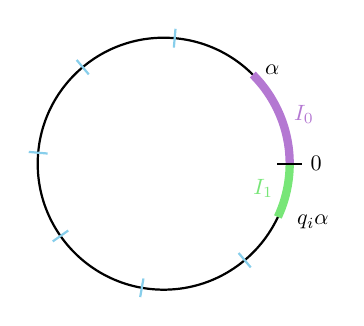
\begin{tikzpicture}[scale=0.8, every node/.style={scale=0.8}]
		\draw[thick] (0,0) circle (2cm);
		% Purple Interval I0
		\draw[line width=3pt, mpur] (0:2cm) arc (0:45:2cm);
		\node[right, mpur] at (22:2.1cm) {$I_0$};
		\node[right] at (45:2.1cm) {$\alpha$};

		% Green Interval I1
		\draw[line width=3pt, mgre] (0:2cm) arc (0:-25:2cm);
		\node[left, mgre] at (-12:1.9cm) {$I_1$};
		\node[right] at (-25:2.2cm) {$q_i \alpha \mod \Z$};

		% Center/Zero mark
		\draw[thick] (1.8cm,0) -- (2.2cm,0) node[right] {0};

		% Orbit ticks
		\foreach \a in {85, 130, 175, 215, 260, 310}
		\draw[mblu, thick] (\a:1.85cm) -- (\a:2.15cm);
	\end{tikzpicture}
\end{minipage}

\smallskip
\begin{lemme}
	If we glue the ends of $I_{0} \cup I_{1}$, $T$ is a rotation.
\end{lemme}

\begin{proof}
	\begin{minipage}[t]{0.55\textwidth}
		\vspace{0pt}
		$T$ acts as an exchange of 2 intervals: this is a rotation on $I_0 \cup I_1$ ``glued''

		Its angle is then $\frac{|I_0|}{|I_0| + |I_1|} = \frac{\alpha}{1 + \alpha - q_1 \alpha}$.

	\end{minipage}
	\hfill
	\begin{minipage}[t]{0.4\textwidth}
		\vspace{0pt}
		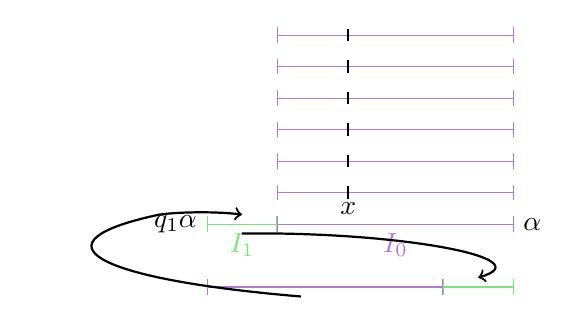
\begin{tikzpicture}[xscale=3, yscale=0.4]
			% --- Upper Stack ---
			\foreach \y in {0,1,...,5} {
					\draw[mpur, |-|] (0,\y+2) -- (1,\y+2);
					\draw[thick] (0.3, \y+1.8) -- (0.3, \y+2.2); % the 'x' mark
				}
			\node[below] at (0.3, 2) {$x$};

			% Bottom row of upper stack
			\draw[mgre, |-|] (-0.3, 1) -- (0, 1) node[midway, below] {$I_1$};
			\draw[mpur, |-|] (0, 1) -- (1, 1) node[midway, below] {$I_0$};
			\node[left] at (-0.3, 1) {$q_1 \alpha$};
			\node[right] at (1, 1) {$\alpha$};

			% Result of exchange
			\draw[mpur, |-|] (-0.3, -1) -- (0.7, -1);
			\draw[mgre, |-|] (0.7, -1) -- (1, -1);

			% Curved arrows for exchange
			\draw[->, bend left=60, thick] (-0.15, 0.7) to (0.85, -0.7);
			\draw[->, bend left=45, thick] (0.1, -1.3) to (-0.5, 1.3) to (-0.15, 1.3);

		\end{tikzpicture}
	\end{minipage}
\end{proof}


\begin{proof}[Proof of 3 gaps Theorem]
	\begin{center}
		\begin{tikzpicture}

			% --- Lower Stack (after text) ---
			\begin{scope}[yshift=-12cm]
				\foreach \y in {0,1,2,3} {
						\draw[mpur, |-|] (0,\y+1) -- (1,\y+1);
					}
				\draw[mgre, |-|] (-0.3, 0) -- (0, 0);
				\draw[mpur, |-|] (0, 0) -- (1, 0);

				\draw[->, thick, mgre] (1.5, 2) -- (2.2, 2);

				% Right side stack
				\begin{scope}[xshift=2.5cm]
					\foreach \y in {0,1,...,6} {
							\draw[mgre, |-|] (0,\y) -- (0.5, \y);
						}
					\foreach \y in {0,1,2,3} {
							\draw[mblu, |-|] (0.5,\y) -- (0.7, \y);
						}
					\node[below] at (0.25, 0) {$I_1$};
					\node[below] at (0.6, 0) {$I_2$};
					\node[left] at (0, 0) {$q_1 \alpha$};
					\node[right] at (0.7, 0) {$q_2 \alpha$};
				\end{scope}
			\end{scope}

		\end{tikzpicture}
	\end{center}

	Let $q_{n+1} = \min \left\{ q > q_{n} \suchthat \norm{q_n \alpha} > \norm{q \alpha} \right\}$ with
	for $x \in S^1$, $\norm{x} = d(x, \Z) \in [0, \frac{1}{2}]$, and $q_{0} = 0$.

\end{proof}

\end{document}
